\documentclass[12pt]{article}

\usepackage{enumerate}
\usepackage{amsmath}
\usepackage{amsthm}
\usepackage{amssymb}
\usepackage{changepage}
\usepackage{graphicx}
\usepackage[a4paper, margin=1in]{geometry}
\allowdisplaybreaks[1]

\title{DATA315 Assignment 3}
\author{Rin Meng 51940633}
\date{\today}

\begin{document}

\maketitle

\begin{enumerate}
    \item
    \begin{verbatim}
source("nickel.R")
acf(nickel, lag.max = 10, 
main = "ACF of Electroless Nickel Concentrations")
    \end{verbatim}
    \begin{center}
        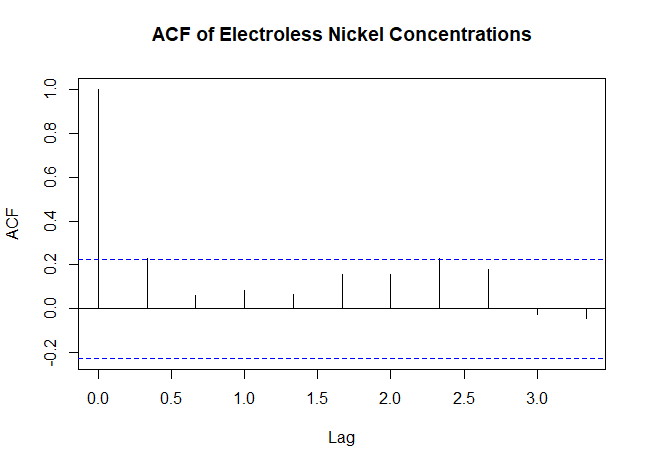
\includegraphics[width=0.8\textwidth]{Rplot.png}
    \end{center}
    The ACF plot seems to follow an MA(1) process,
    as significant correlation at lag 1 followed by immediate drop to near zero. 
    \item
\begin{verbatim}
data(lynx)
acf(lynx, lag.max = 10, main = "ACF of Lynx Trapping Data")
\end{verbatim}
    \begin{center}
        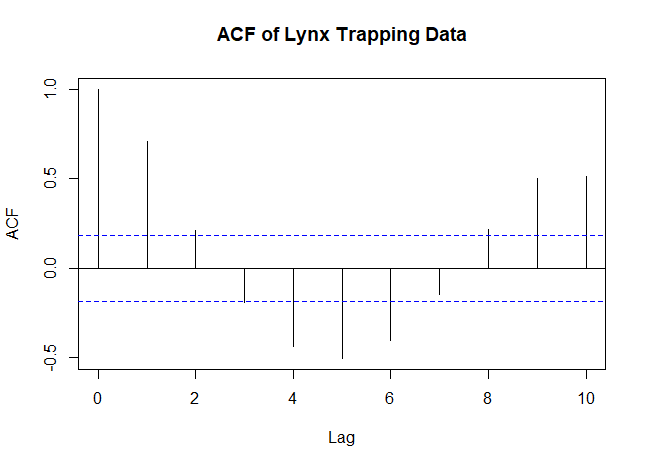
\includegraphics[width=0.8\textwidth]{Rplot01.png}
    \end{center}
    So far, there are no models that fit, because the plot shows a cyclic pattern between
    predator and prey populations. 
    \item
\begin{verbatim}
source("Globaltemps.R")
temps <- ts(temps, start = 1880, end = 2016)
acf(temps, lag.max = 10, 
main = "ACF of Global Average Temperatures")
\end{verbatim}
    \begin{center}
        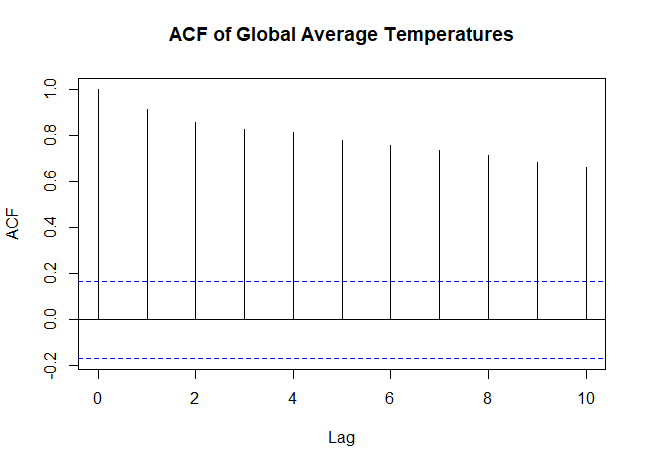
\includegraphics[width=0.8\textwidth]{Rplot02.png}
    \end{center}
    The ACF plot seems to follow an AR(1) process,
    as significant correlation at lag 1 followed by gradual decay.
    \item 
    \begin{verbatim}
data("EuStockMarkets")
dax <- EuStockMarkets[, 1]
dax_ts <- ts(dax, start = c(1991, 1), frequency = 260)
# 260 trading days per year

plot(dax_ts, 
main = "DAX Stock Index Time Series", 
ylab = "Index Value", xlab = "Year", 
col = "blue", type = "l") # Time series plot

acf(dax_ts, main = "ACF of DAX Stock Index") # ACF plot

log_dax <- log(dax_ts)          # Take the natural log
diff_log_dax <- diff(log_dax)   # Compute first differences (log returns)

    \end{verbatim}
    \begin{center}
        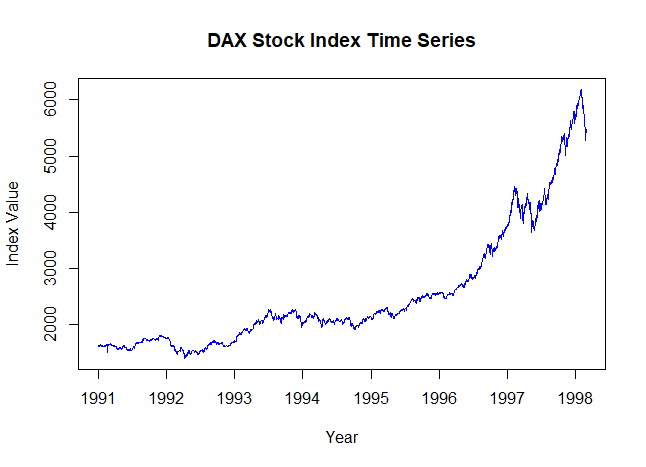
\includegraphics[width=0.8\textwidth]{Rplot03.png}
        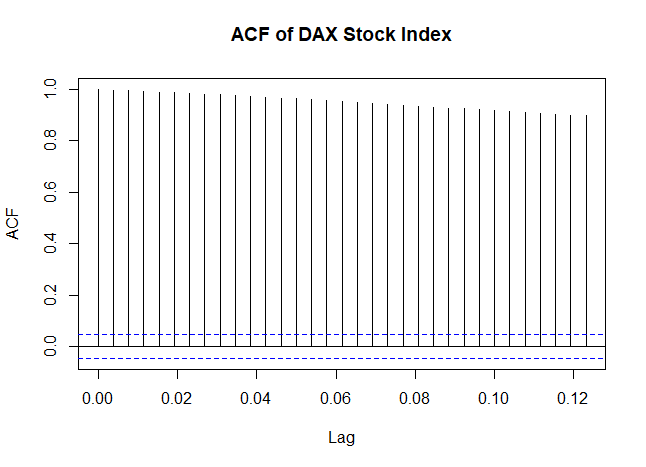
\includegraphics[width=0.8\textwidth]{Rplot04.png}
        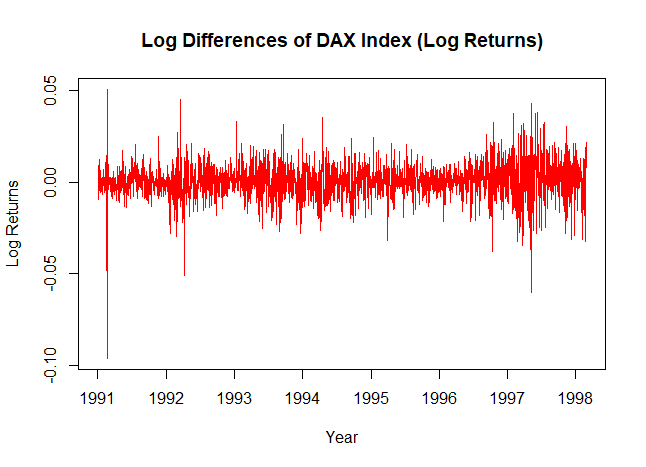
\includegraphics[width=0.8\textwidth]{Rplot05.png}
    \end{center}
    Some observations for the DAX stock index time series plot; visually, we can see that
    there is a general upward trend with some fluctuations. The ACF plot shows that there is
    a significant correlation at lag 1, followed by a gradual, slow decay, which means that it
    may be following other process we have not covered yet. The log returns plot shows that 
    the data revolves around 0, which is a good sign for stationarity.


\end{enumerate}


\end{document}
